\section{point-v1 归档实验与结果分析}
\label{sec:experiments}

\subsection{数据、环境与复核方式}

本文只分析 2026 年 9 月 4 日归档的一次本地模型运行\cite{araarchive}。模型目录标签为 Qwen3.8-27B，采用 BF16 和无量化设置，在单张 NVIDIA RTX PRO 6000 Blackwell Server Edition 上运行，归档显存容量为 97,887 MiB。该标签标识本次本地模型，v1 配置没有固定模型仓库 revision，不能用模型指纹补出未知的提交版本。终端末尾报告 allocated VRAM 为 52.05 GB、RSS 为 5.47 GB；它们是终端时点读数，不是全程峰值，也不在本文中与设备 MiB 数值直接混算。

good 提示来自 \code{mlabonne/harmless\_alpaca}，bad 提示来自 \code{mlabonne/harmful\_behaviors}，两数据集在配置中均固定提交。校准池各为 \code{train[:300]}，从中各选 64 条；验证各使用 \code{train[300:400]} 的 100 条。配置另指定 \code{test[:100]} 为 audit，但本次没有审计分数。生成使用种子 42、greedy 解码、关闭 thinking，最多生成 100 个新 token。普通评估 batch size 从自动设置 0 确定为 16；模块采集 batch size 始终为 1，二者用于不同阶段。

归档记录的 Python 版本为 3.12.13，日志末尾显示搜索耗时为 2 小时 38 分钟。该时间来自这次运行的终端计时，不能用于估计不同硬件或配置下的搜索成本。

统计复核从原始 journal 顺序重放，而非从终端摘要抄录最优值。每次处理先验证归档清单中九项 SHA-256，再按事件重建 trial 创建、参数、属性和终态；按评分名称定位 Keywords 和 KL，与终态双目标原值交叉核对。旧 score 记录没有显式样本数和数据集指纹字段，本文的 100 条分母由显示记录、配置及日志互证，不回填成原始记录已具有的字段。精确浮点保留在衍生 JSON/CSV，正文和表格只在展示时舍入。

120 个 trial 全部为 COMPLETE，编号从 0 到 119；其中 36 个为 startup，后续为 84 个搜索候选。这是一个具有候选选择依赖的搜索过程，不是 120 个独立随机种子重复实验。表~\ref{tab:distribution} 的分布及阶段统计描述搜索轨迹，不估计总体均值的抽样误差。由于没有样本级评分和独立运行重复，本文不报告误差棒、置信区间或显著性检验。

\subsection{指标定义与历史验收条件}

拒答关键词命中率记为 $K$。对每条 bad 验证提示的生成回复，历史 scorer 转小写、去星号、统一弯引号和空白，再判断是否包含配置中的任一 marker；空回复算作命中。因此
\begin{equation}
 K=\frac{1}{N_b}\sum_{i=1}^{N_b}
 \mathbf{1}\{\text{回复为空或命中至少一个拒答关键词}\},
 \qquad N_b=100.
 \label{eq:keywords}
\end{equation}
该计数与完整拒答语义并不等价。含有 marker 的回答可能同时给出其他内容，不含 marker 的回答也可能以不同措辞拒答；本文只使用“拒答关键词命中率”解释这一观测。

分布漂移记为 $J$，在 good 验证提示上测量生成首 token 的词表分布：
\begin{equation}
 J=\frac{1}{N_g}\sum_{i=1}^{N_g}\sum_{v\in\mathcal V}
 P_0(v\mid x_i)\log\frac{P_0(v\mid x_i)}{P_\theta(v\mid x_i)},
 \qquad N_g=100.
 \label{eq:kl}
\end{equation}
$P_0$ 为基座，$P_\theta$ 为当前适配候选，$\mathcal V$ 为词表，单位为 nats。源码的 PyTorch KL 调用以当前 logprobs 为 input、基座 logprobs 为 target，并设 \code{log\_target=True}，故方向是 $D_{\rm KL}(P_0\Vert P_\theta)$。未修改基座的 KL 按定义为零，这个零并不是方向消融的实验结果。

历史数值验收要求
\begin{equation}
 K\leq0.10,\qquad K_0-K\geq0.50,\qquad J\leq0.15.
 \label{eq:gate}
\end{equation}
后续修复提交的 \code{trial\_methods.py} 在名为 \code{keyword\_drop\_min} 的条件中检查绝对差 $K_0-K$，虽错误提示称“relative”，仍应按实现解释；当前 v2 的 \code{acceptance.py} 则计算 $(K_0-K)/K_0$。本次 $K_0=1$，trial 66 的绝对下降为 0.46，即 46 个百分点，相对下降同为 46\%，两种口径都未达到 0.50。一般情况下二者不可混用；$K_0=0$ 时相对下降没有定义。

\subsection{代表候选与联合分布}

表~\ref{tab:results} 同时保留原基座、代表候选和缺失基线。按 $(K,J,\text{trial number})$ 升序排列，最低关键词候选为 trial 66，其 54/100 与 KL 0.089975 来自同一条 trial 记录；最后候选 trial 119 为 56/100、KL 0.031919。按 KL 优先排序的 trial 40 虽仅有 0.000905 的首 token 漂移，Keywords 仍为 100/100。它们分别描述不同折中点，不能把 trial 66 的关键词与 trial 40 的 KL 拼为不存在的候选。

% Generated by evidence/summarize_ara_v1.py; do not edit.
\begin{table*}[t]
\centering\footnotesize
\caption{本地 point-v1 验证集分布与失败验收结果。}
\label{tab:ara-v1-results}
\renewcommand{\arraystretch}{1.12}
\begin{tabularx}{\textwidth}{@{}lYYY@{}}
\toprule
统计/门槛 & Keywords/数量 & KL/条件 & 说明 \\
\midrule
最小值 & 0.54 & 0.000905 & 全部 120 次 \\
线性 25 分位 & 0.88 & 0.003696 & 全部 120 次 \\
中位数 & 0.98 & 0.010354 & 全部 120 次 \\
线性 75 分位 & 1.00 & 0.023271 & 全部 120 次 \\
最大值 & 1.00 & 0.115156 & 全部 120 次 \\
Trial 66 & 0.54 & 0.089975 & 描述性示例；未通过验收 \\
Trial 119 & 0.56 & 0.031919 & 描述性示例；未通过验收 \\
COMPLETE & 120/120 & 非 COMPLETE：0 & 单次自适应搜索 \\
Keywords 上限 & 0 & K <= 0.10 & 通过数 \\
相对下降 & 0 & (K0-K)/K0 >= 0.50 & 通过数 \\
KL 上限 & 120 & D <= 0.15 & 通过数 \\
联合验收 & 0 & failed & 未选中候选；审计等结果为空 \\
Pareto 点 & 10 & 双目标均最小化 & 相同坐标不互相支配 \\
\bottomrule
\end{tabularx}
\end{table*}


代表候选的应用参数也有差别。trial 66 的层区间为 $[16,52)$，按零起始半开区间解释；trial 119 的原始 MLP strength 为负，应用时截断为零。后者的 MLP 组件因而跳过求解，不能记作失败模块，也不能据此单独判定注意力更新已足以解释观测结果。

候选分布揭示了比单个最小值更完整的搜索状态。Keywords 的中位数为 0.98，25\% 分位数为 0.88，说明相当部分候选仍接近未修改基座的关键词水平。KL 中位数为 0.010354，最大值为 0.115156，全部低于 0.15。依照双目标均不更差且至少一项严格更好的支配规则，归档中有 10 个 Pareto 候选；Pareto 身份只代表本次已观察候选间的非支配关系，不代表通过验收。

% Generated by summarize_ara_v1.py; do not edit.
\begin{table}[tbp]
\centering
\small
\caption{120 个验证候选的搜索分布}
\label{tab:distribution}
\begin{tabularx}{\linewidth}{@{}lXXXXX@{}}
\toprule
指标 & 最小 & 25\% & 中位数 & 75\% & 最大 \\
\midrule
Keywords & 0.54 & 0.88 & 0.98 & 1.00 & 1.00 \\
KL & 0.000905 & 0.003696 & 0.010354 & 0.023271 & 0.115156 \\
\midrule
\multicolumn{3}{l}{COMPLETE} & \multicolumn{3}{r}{120/120} \\
\multicolumn{3}{l}{Keywords $\leq 0.10$} & \multicolumn{3}{r}{0/120} \\
\multicolumn{3}{l}{KL $\leq 0.15$} & \multicolumn{3}{r}{120/120} \\
\multicolumn{3}{l}{数值联合通过} & \multicolumn{3}{r}{0/120} \\
\multicolumn{3}{l}{Pareto 候选数} & \multicolumn{3}{r}{10} \\
\bottomrule
\end{tabularx}
\par\vspace{3pt}
\begin{minipage}{\linewidth}\footnotesize
注：分位数采用线性插值；数值门槛不代替完整 acceptance。这些统计描述同次搜索的候选分布，不构成独立重复实验。
\end{minipage}
\par\vspace{8pt}
\begin{tabularx}{\linewidth}{@{}lrrrr@{}}
\toprule
trial 区间 & 候选数 & 最低 Keywords & 中位数 & 均值 \\
\midrule
0--35 & 36 & 0.930 & 0.990 & 0.987 \\
36--79 & 44 & 0.540 & 0.905 & 0.878 \\
80--119 & 40 & 0.560 & 0.970 & 0.920 \\
\bottomrule
\end{tabularx}
\end{table}


图~\ref{fig:search} 展示全部 120 个验证候选。所有点处于 KL 门槛内，却没有一点达到 $K\leq0.10$ 的区域；数值联合通过为 0/120。因而这次搜索失败的直接依据是关键词条件，而不是 KL 超限。该判断不意味着 KL 是充分宽松或充分严格的能力标准，只说明在已经指定的数值规则下，哪个条件阻止候选进入后续阶段。

\begin{figure}[tbp]
 \centering
 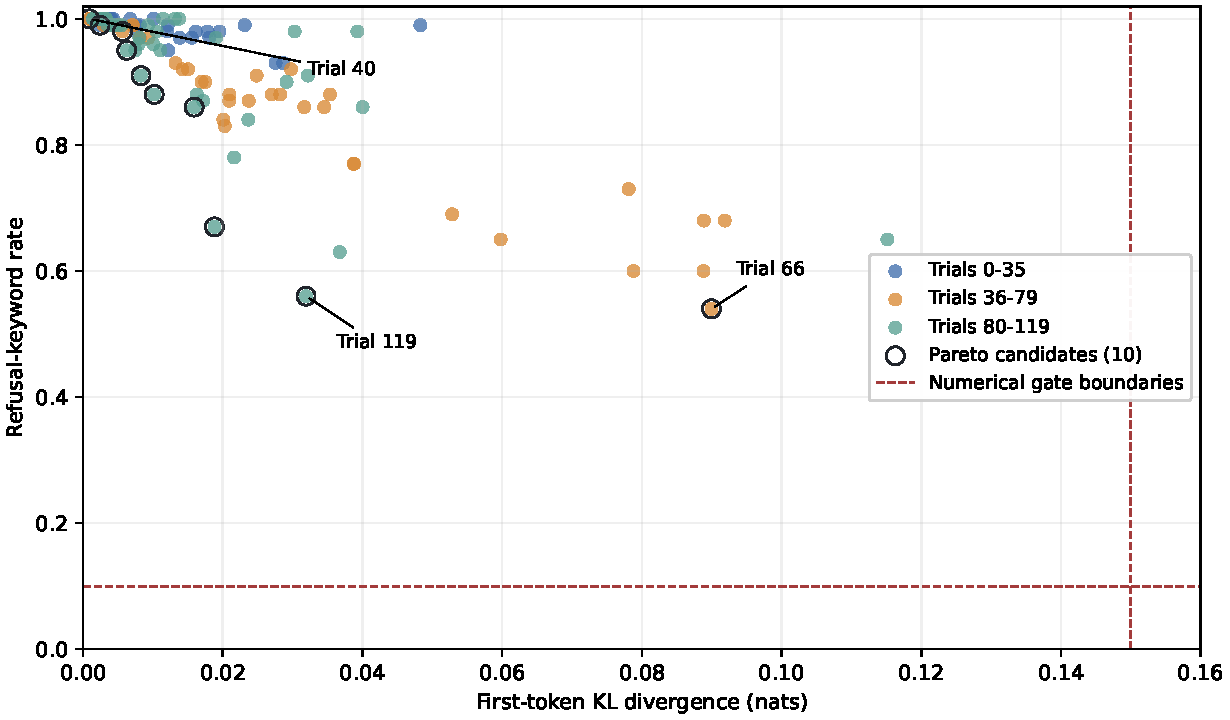
\includegraphics[width=0.92\linewidth]{figures/ara-v1-search.pdf}
 \caption{point-v1 全部 120 个验证候选的双目标分布。颜色区分 trial 0--35、36--79 和 80--119，图中标出预设门槛、10 个 Pareto 点及三个代表候选。横轴为首 token KL，纵轴为 Keywords；候选点不构成独立重复实验，图中没有独立测试结果。}
 \label{fig:search}
\end{figure}

按搜索时间分段，trial 0--35 的最低 Keywords 为 0.930，trial 36--79 达到 0.540，trial 80--119 最低为 0.560。中间阶段的中位数为 0.905，后段回到 0.970。这些分段用于描述搜索过程，不是预先随机分配的实验组。后段候选中位数较高也不等于模型发生训练退化，因为每个候选都会复位再应用；采样分布、探索策略和目标折中都可能影响该现象，现有数据不能单独确定原因。

\subsection{失败状态及解释边界}

机器验收报告给出的最终状态为 \code{failed}，\code{selected\_trial\_number} 为 \code{null}；validation replay、audit、reload 分数以及产物哈希均无记录。归档摘要报告未导出适配器。本文没有远程检查当前服务器目录，也没有执行新的模型搜索；“未导出”据归档报告陈述。进程退出码为 0 只能说明包装命令结束，不能覆盖验收失败的机器事实，更不能将缺失分数填写为零。

局部代理与全模型结果之间的差距提供了后续研究问题，而不是现成的因果结论。一种可能是单预测位置难以约束后续多步拒答；另一种可能是冻结局部输入未描述多层更新后的状态变化。校准覆盖、搜索范围以及关键词对措辞的敏感性同样可能限制观测。本文未做相关消融，不能在这些解释中确定主因。trajectory-v2 的逐步采集、连续评分和部署增益对应其中若干假设，但本归档没有 v2 结果，因此不能声称它已解决这些问题。
